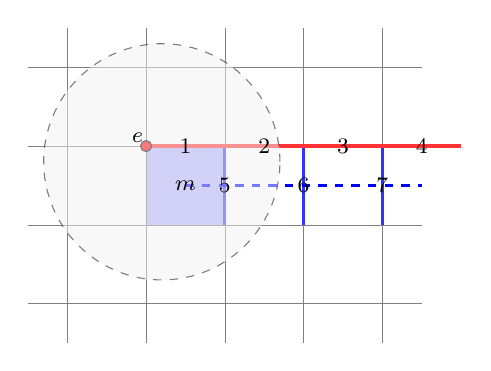
\begin{tikzpicture}[node font=\footnotesize]
  \draw [step=1, help lines]
    (-1.5,-1.5) grid (3.5,2.5);
  % m particle
  \draw [help lines, fill=blue!30]
    (0,0) rectangle (1,1) node [midway] (m) {};
  \foreach \x in {1,2,3}
    \draw [very thick, blue!80] (\x,0) -- (\x,1);
  \draw [thick, dashed, blue] (0.5,0.5) -- (3.5,0.5);
  % e particle
  \draw [very thick, red!80] (0,1) -- (4,1);
  \draw [fill=red] (0,1) circle (0.07) node [above left] (e) {};
  % local region
  \draw [dashed, fill=gray!10, opacity=0.5] (0.2,0.8) circle (1.5);
  % labels
  \node at (e) {$e$};
  \node at (m) {$m$};
  \foreach \x/\xtext in {0.5/1, 1.5/2, 2.5/3, 3.5/4}
    \node at (\x,1) {$\xtext$};
  \foreach \x/\xtext in {1/5, 2/6, 3/7}
    \node at (\x,0.5) {$\xtext$};
\end{tikzpicture}
